\documentclass{article}
\usepackage{graphicx} % Required for inserting images



\begin{document}
\section*{Logic Gate Simulation Documentation}

\subsection*{Introduction}

The logic gate simulation allows users to model and simulate digital circuits using logic gates. The simulation process includes the ability to connect multiple gates, synchronize operations using a clock, and control the simulation by advancing one clock cycle or running continuously.

\subsection*{Simulation Components}

The simulation involves the following components:

\begin{itemize}
    \item \textbf{Logic Gates}: Basic building blocks representing logical operations.
    \item \textbf{Clock}: Synchronization mechanism to control the simulation.
\end{itemize}

\subsection*{Simulation Process}

The simulation process follows these steps:

\begin{enumerate}
    \item \textbf{Initialization}: Create and arrange logic gates within the simulation environment.
    \item \textbf{Connection}: Connect the output of one gate to the input of another to model logical relationships.
    \item \textbf{Clock Configuration}: Set the clock frequency and parameters for synchronization.
    \item \textbf{Simulation Run}:
        \begin{itemize}
            \item \textbf{Single Clock Cycle}: Advance the simulation by one clock cycle to observe changes.
            \item \textbf{Continuous Run}: Allow the simulation to run continuously, updating with each clock cycle.
        \end{itemize}
\end{enumerate}



\section*{Classes Descriptions}

\subsection*{Port Class Description}

\subsubsection*{Port\_Kind}
An enum representing different kinds of ports, categorized as input (\texttt{in}) or output (\texttt{out}).

\subsubsection*{Port}
A structure representing a circle-shaped port with specified coordinates and type (IN/OUT).

\begin{itemize}
    \item \texttt{List<Port*> connections} - List of connections to other ports.
    \item \texttt{Vec2 coordinates} - Coordinates of the center of the port.
    \item \texttt{f32 radius} - Radius of the port.
    \item \texttt{Port\_Kind kind} - Kind of port (input or output).
    \item \texttt{Gate* gate} - Pointer to the gate to which the port belongs.
\end{itemize}

\subsubsection*{Functions}

\begin{itemize}
    \item \texttt{Port(Vec2 coordinates, Port\_Kind type, Gate* gate)} - Initializes a circle-shaped port with specified coordinates and type.
    \item \texttt{void move(Vec2 offset)} - Moves the port by the given offset.
    \item \texttt{void add\_connection(Port* new\_port)} - Connects the port to another specified port.
    \item \texttt{void remove\_connection(Port* old\_port)} - Disconnects the port from a specified connected port.
    \item \texttt{void remove\_all\_connections()} - Disconnects the port from all connected ports.
    \item \texttt{Vec2 get\_coordinates() const} - Gets the coordinates of the port.
    \item \texttt{bool is\_under\_mouse(Vec2 mouse\_position) const} - Checks if the port is under the specified mouse position.
\end{itemize}

\subsection*{Gate Class Description}

\subsubsection*{Gate\_Kind}
An enum representing different kinds of logic gates: AND, OR, XOR, NAND, NOR, XNOR and NOT.



\subsubsection*{Gate}
A structure representing a gate.

\begin{itemize}
    \item \texttt{Array<Port*> in\_ports} - List of input ports.
    \item \texttt{Array<Port*> out\_ports} - List of output ports.
    \item \texttt{math::Vec2 coordinates} - Coordinates of the top-left corner of the gate.
    \item \texttt{math::Vec2 dimensions} - Dimensions of the gate (width and height).
    \item \texttt{Gate\_Kind kind} - Kind of logic gate.
    \item \texttt{Evaluation\_State evaluation} - State of gate evaluation.
\end{itemize}

\subsubsection*{Functions}

\begin{itemize}
    \item \texttt{Gate(math::Vec2 dimensions, math::Vec2 coordinates, Gate\_Kind kind)} - Constructs a new gate.
    \item \texttt{void move(math::Vec2 offset)} - Moves the gate to a new location.
\end{itemize}

\subsection*{Evaluator Class Description}

\subsubsection*{Functions}

\begin{itemize}
    \item \texttt{void evaluate(List<Gate>\& gates)} - Evaluates the logic gates in the given list.
\end{itemize}

\subsubsection*{Helper Functions}

\begin{itemize}
    \item \texttt{static bool get\_input\_value(Port* const port)} - Gets the input value for a port.
\end{itemize}

\begin{figure}[h]
    \centering
    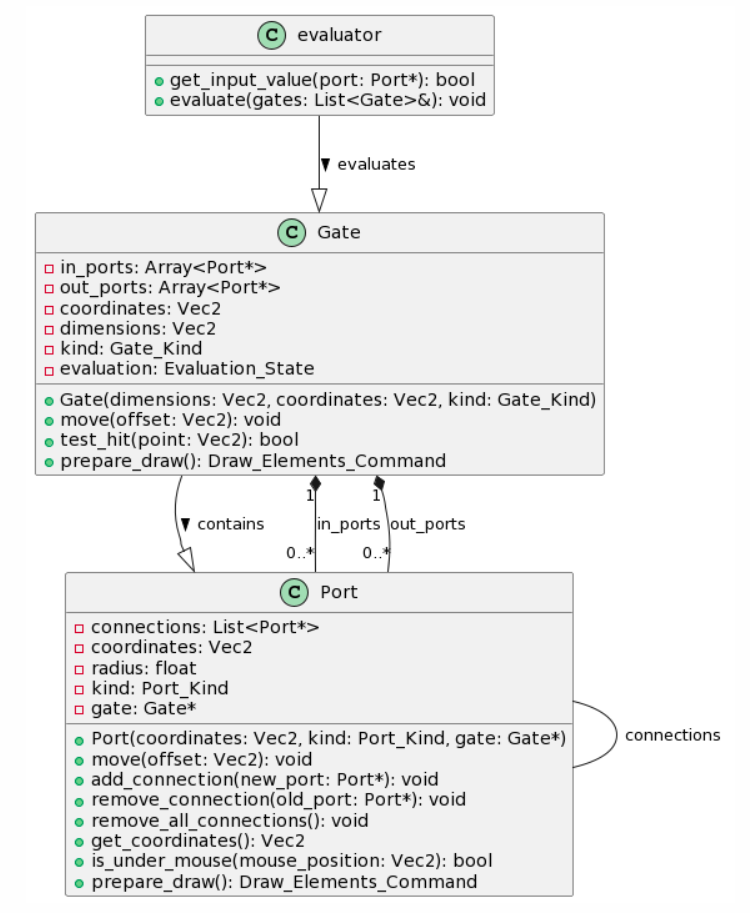
\includegraphics[width=1\textwidth]{diagramklas.png}
    \caption{Class diagram of the logic gate simulation.}
    \label{fig:class_diagram}
\end{figure}
\end{document}

